% !TeX root = ../main.tex

%\section{Simulation Study}

\subsection{Data Simulation}

To test the CarHHMM with STFT, 500 separate sequences of 100 marine-mammal dives were simulated. The coarse-scale observations $Y$ were set as the duration of each dive, and the fine-scale observations $Y^*$ were set as one-dimensional acceleration readings simulated at 50 hertz. The number of possible states for both the coarse- and fine- scale Markov chains was set to 2, i.e. $N = N^* = 2$. 

On the coarse scale, the following parameters were used:
$$\Gamma = \begin{pmatrix} 0.5 & 0.5 \\ 0.5 & 0.5 \end{pmatrix} $$
$$Y_t|X_t \sim \rm{Gamma} $$
\begin{align*}
	&\bbE(Y_t|X_t = 1) = 15 s &\bbE(Y_t|X_t = 2) = 60 s \\
	%
	&\bbV(Y_t|X_t = 1) = 25 s^2 &\bbV(Y_t|X_t = 2) = 100 s^2
\end{align*}
Once the coarse-scale dive durations were calculated for $t = 1, \ldots, 100$, dive $t$ was broken into $\lfloor Y_t/2 \rfloor$ 2-second segments (the end of the dive sequence was discarded). Each 2-second segment was assigned a behaviour according to a fine-scale Markov chain $X^*_t$, where the parameters were set as follows:
%
$$\Gamma^{*(1)} = \begin{pmatrix} 0.5 & 0.5 \\ 0.9 & 0.1 \end{pmatrix} \qquad 	\Gamma^{*(2)} = \begin{pmatrix} 0.8 & 0.2 \\ 0.3 & 0.7 \end{pmatrix}$$
%
where $\Gamma^{*(1)}$ was used for dives where $X_t = 1$ and $\Gamma^{*(2)}$ was used for dives where $X_t = 2$. For each 2-second segment, the Fourier modes $\hat{Y}^*_{t,s^*} \in \mathbb{C}^{100}$ were simulated such that $Z^{*(1)}_{t,s^*}$ and $Z^{*(2)}_{t,s^*}$ would have the following distributions: 

\begin{align*}
    \left(Z^{*(1)}_{t,s^*} | Z^{*(1)}_{t,s^*-1}, X^*_{t,s^*} = 1 \right) &\sim \mathcal{N} \left(\phi^{*(1)}Z^{*(1)}_{t,s^*-1} + \phi^{*(1)}\mu^{*(1)}, (\sigma^{*(1)})^2 \right) \\
    %
    \left(Z^{*(1)}_{t,s^*} | Z^{*(1)}_{t,s^*-1}, X^*_{t,s^*} = 2 \right) &\sim \mathcal{N} \left(\phi^{*(2)}Z^{*(1)}_{t,s^*-1} + \phi^{*(2)}\mu^{*(2)}, (\sigma^{*(2)})^2 \right) \\
    %
    \mu^{*(1)} = 0.0,\enspace \sigma^{*(1)} &= 0.05,\enspace \phi^{*(1)} = 0.99 \\
    %
    \mu^{*(2)} = 0.0,\enspace \sigma^{*(2)} &= 0.1,\enspace \phi^{*(2)} = 0.95 \\\\
    %
    \left(Z^{*(2)}_{t,s^*} | X^*_{t,s^*} = 1\right) &\sim {\rm{Gamma}}\left(\alpha^{*(1)}, \beta^{*(1)} \right) \\
    %
    \left(Z^{*(2)}_{t,s^*} | X^*_{t,s^*} = 2\right) &\sim {\rm{Gamma}}\left(\alpha^{*(2)}, \beta^{*(2)} \right) \\
    %
    \alpha^{*(1)} = 10.10, \enspace & \enspace \beta^{*(1)} = 1.00 \\
    %
    \alpha^{*(2)} = 305.94, \enspace & \enspace \beta^{*(2)} = 1.00
\end{align*}
%
See the appendix for more details regarding the simulation procedure for $\hat Y^*$. The emission distribution of the 2-second average acceleration $Z_{t,s^*}^{*(1)}$ in particular can be reparameterized as an OU process according to theorem 1:
%
$$dZ^{*(1)}_{t,s^*} = \beta^*(\gamma^* - Z^{*(1)}_{t,s^*})dt^* + \omega^* dW_{t,t^*}$$
%
$$\gamma^{*(1)} = 0, \enspace \beta^{*(1)} = -\frac{\log(\phi^{*(1)})}{\Delta t^*} = 0.0111, \enspace \omega^{*(1)} = \sqrt{\frac{2(\sigma^{^{*(1)}})^2\log(\phi^{*(1)})}{\Delta t^* ((\phi^{*(1)})^2-1)}} = 0.0355$$
$$\gamma^{*(2)} = 0, \enspace \beta^{*(2)} = -\frac{\log(\phi^{*(2)})}{\Delta t^*} = 0.0256, \enspace \omega^{*(2)} = \sqrt{\frac{2(\sigma^{*(2)})^2\log(\phi^{*(2)})}{\Delta t^* ((\phi^{*(2)})^2-1)}} = 0.7625$$

A visualization of the first 5 dives of one simulated data set can be seen in (fig. \ref{fig:sim_data}).

\begin{figure}[!ht]
	\centering
	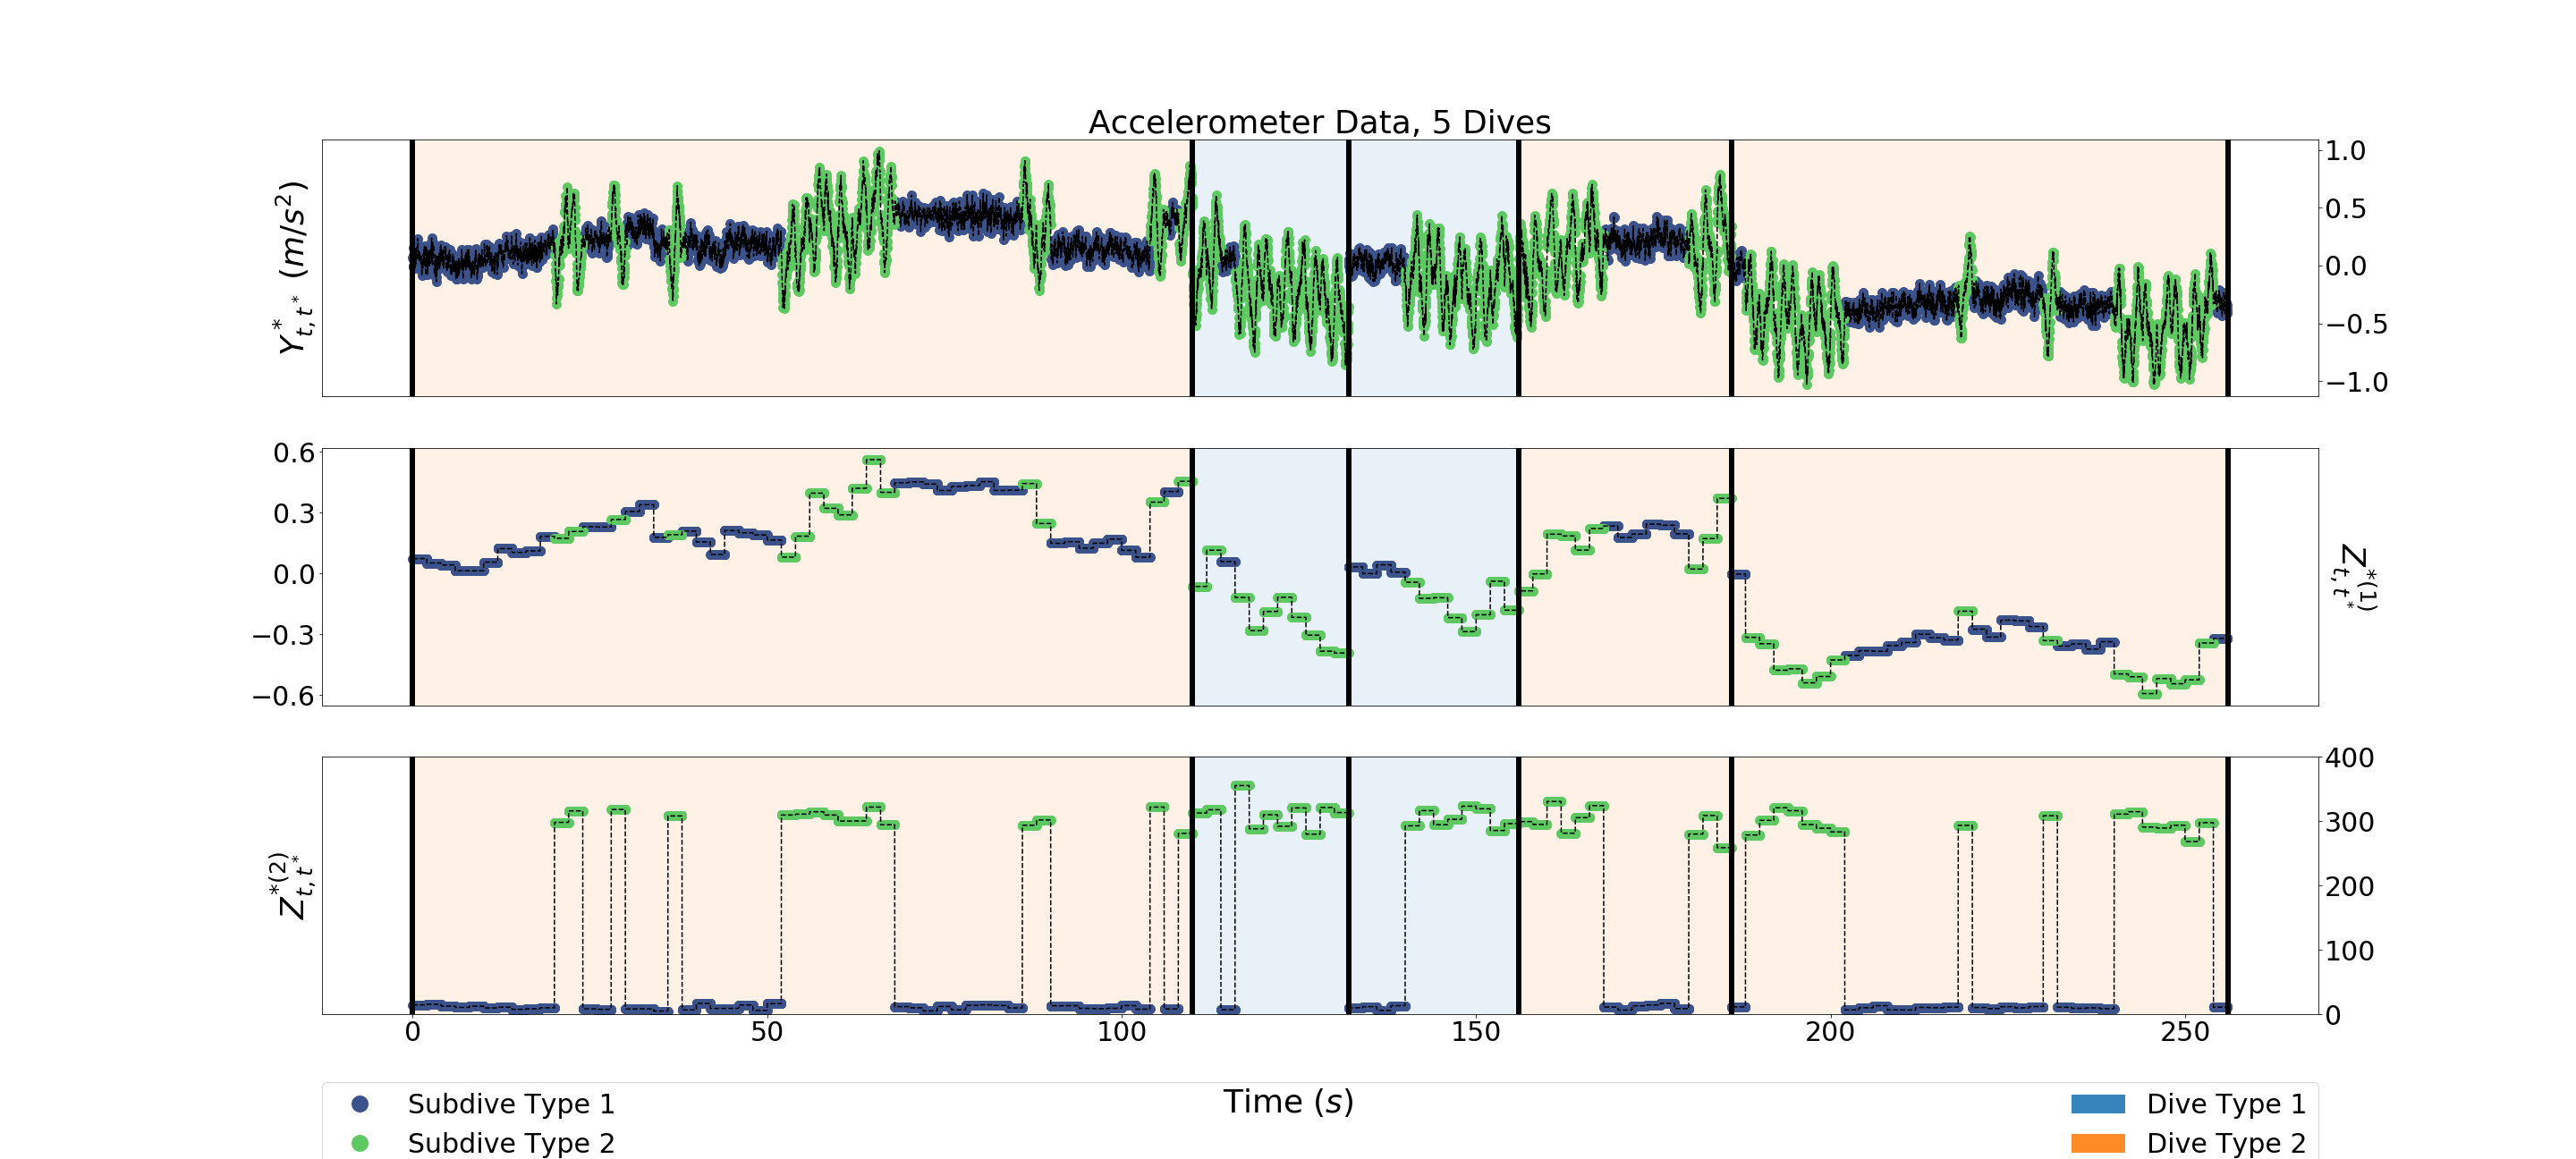
\includegraphics[width=5in]{../Plots/sim_data.png}
	\caption{Simulated acceleration data for one dive. The color of the line corresponds to the true fine-scale state of the sub-dive process, while the color of the background corresponds to the true dive type of the simulated whale, where blue corresponds to dive type 1 and orange corresponds to dive type 2.}
	\label{fig:sim_data}
\end{figure}


\subsection{Simulation Results}

Four different models were fit to each simulated data set:

\begin{enumerate}
    \item A CarHMM with no hierarchical structure using both $Z^{*(1)}$ and $Z^{*(2)}$ as fine-scale observations (\textbf{CarHMM}).
    \item An HHMM with no auto-correlation using both $Z^{*(1)}$ and $Z^{*(2)}$ as fine-scale observations (\textbf{HHMM}).
    \item A CarHHMM using $Z^{*(1)}$, but NOT $Z^{*(2)}$ as fine-scale observations (\textbf{CarHHMM1}). To ensure that the CarHHMM could still see the ``wigliness" of the process, we halved the window size to 1 second for the CarHHMM1.
    \item A CarHHMM using both $Z^{*(1)}$ and $Z^{*(2)}$ as fine-scale observations (\textbf{CarHHMM2}).
\end{enumerate}
%
The purpose of including each of these models is to leave one important aspect of the full model (CarHHMM2) out of each of the preceding three and observe the effects on a simulated data set. In particular, the CarHMM lacks a hierarchical structure, the HHMM is missing auto-correlation within the fine-scale observations, and the CarHHMM1 does not have $Z^{*(2)}$ as observations.

%%% Accuracy %%%
Every model was able to decode the fine-scale hidden states of the process effectively perfectly except for the CarHHMM1, which did not have access to the Fourier modes $Z^{*(2)}$. This is intuitively clear because the fine-scale states are much more distinct in their Fourier modes than in their average acceleration. For the coarse-scale hidden state, the CarHMM lacked a hierarchical structure and could not make any predictions at all. The other three models all achieved an accuracy of approximately 90\%, with the CarHHMM slightly more likely to categorize a dive as dive type 2 than the other models. (Fig. \ref{fig:acc}) shows the decoded state probabilities of both the fine and coarse hidden states for the first 10 dives of one simulated data set. (Tbl. \ref{table:accuracy}) also lists more details regarding the accuracy and training times of each model for each true dive and sub-dive state.

\begin{figure}[t!]
    \centering
    \begin{subfigure}{1.0\textwidth}
        \centering
        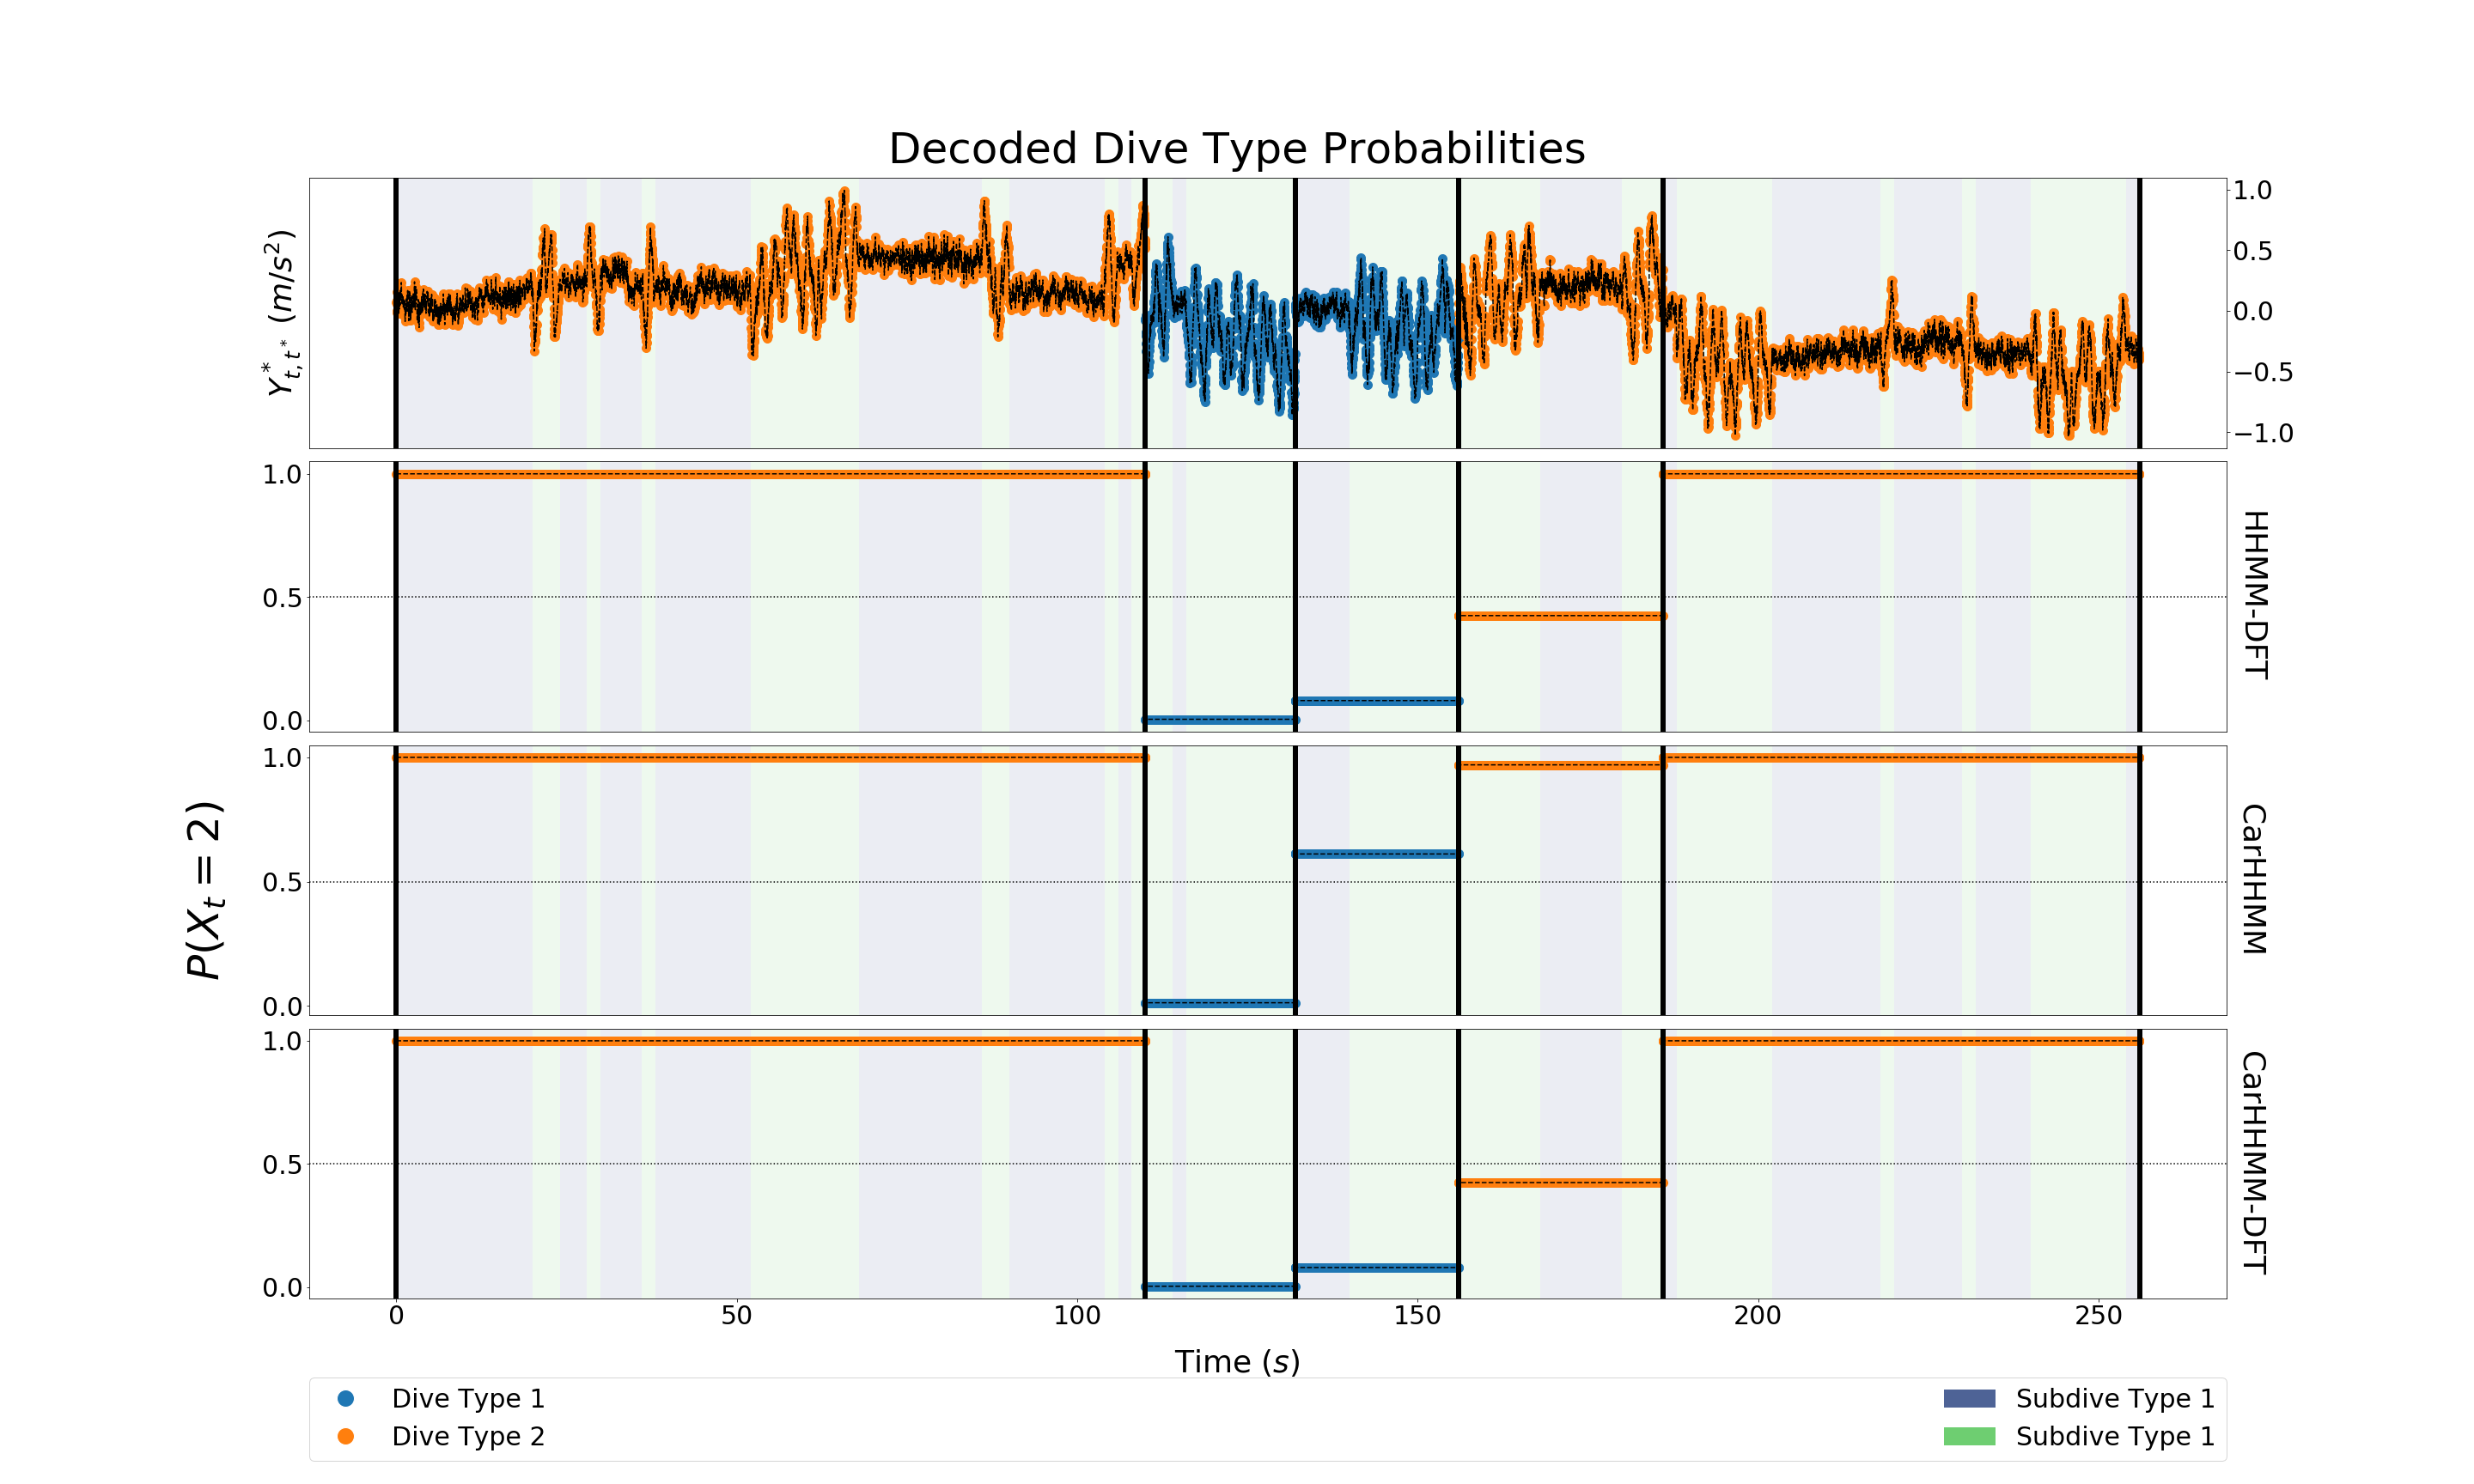
\includegraphics[width=5in]{Plots/Posterior_Coarse_States.png}
        \caption{Coarse-scale hidden process}
    \end{subfigure}
    \newline
    \begin{subfigure}{1.0\textwidth}
        \centering
        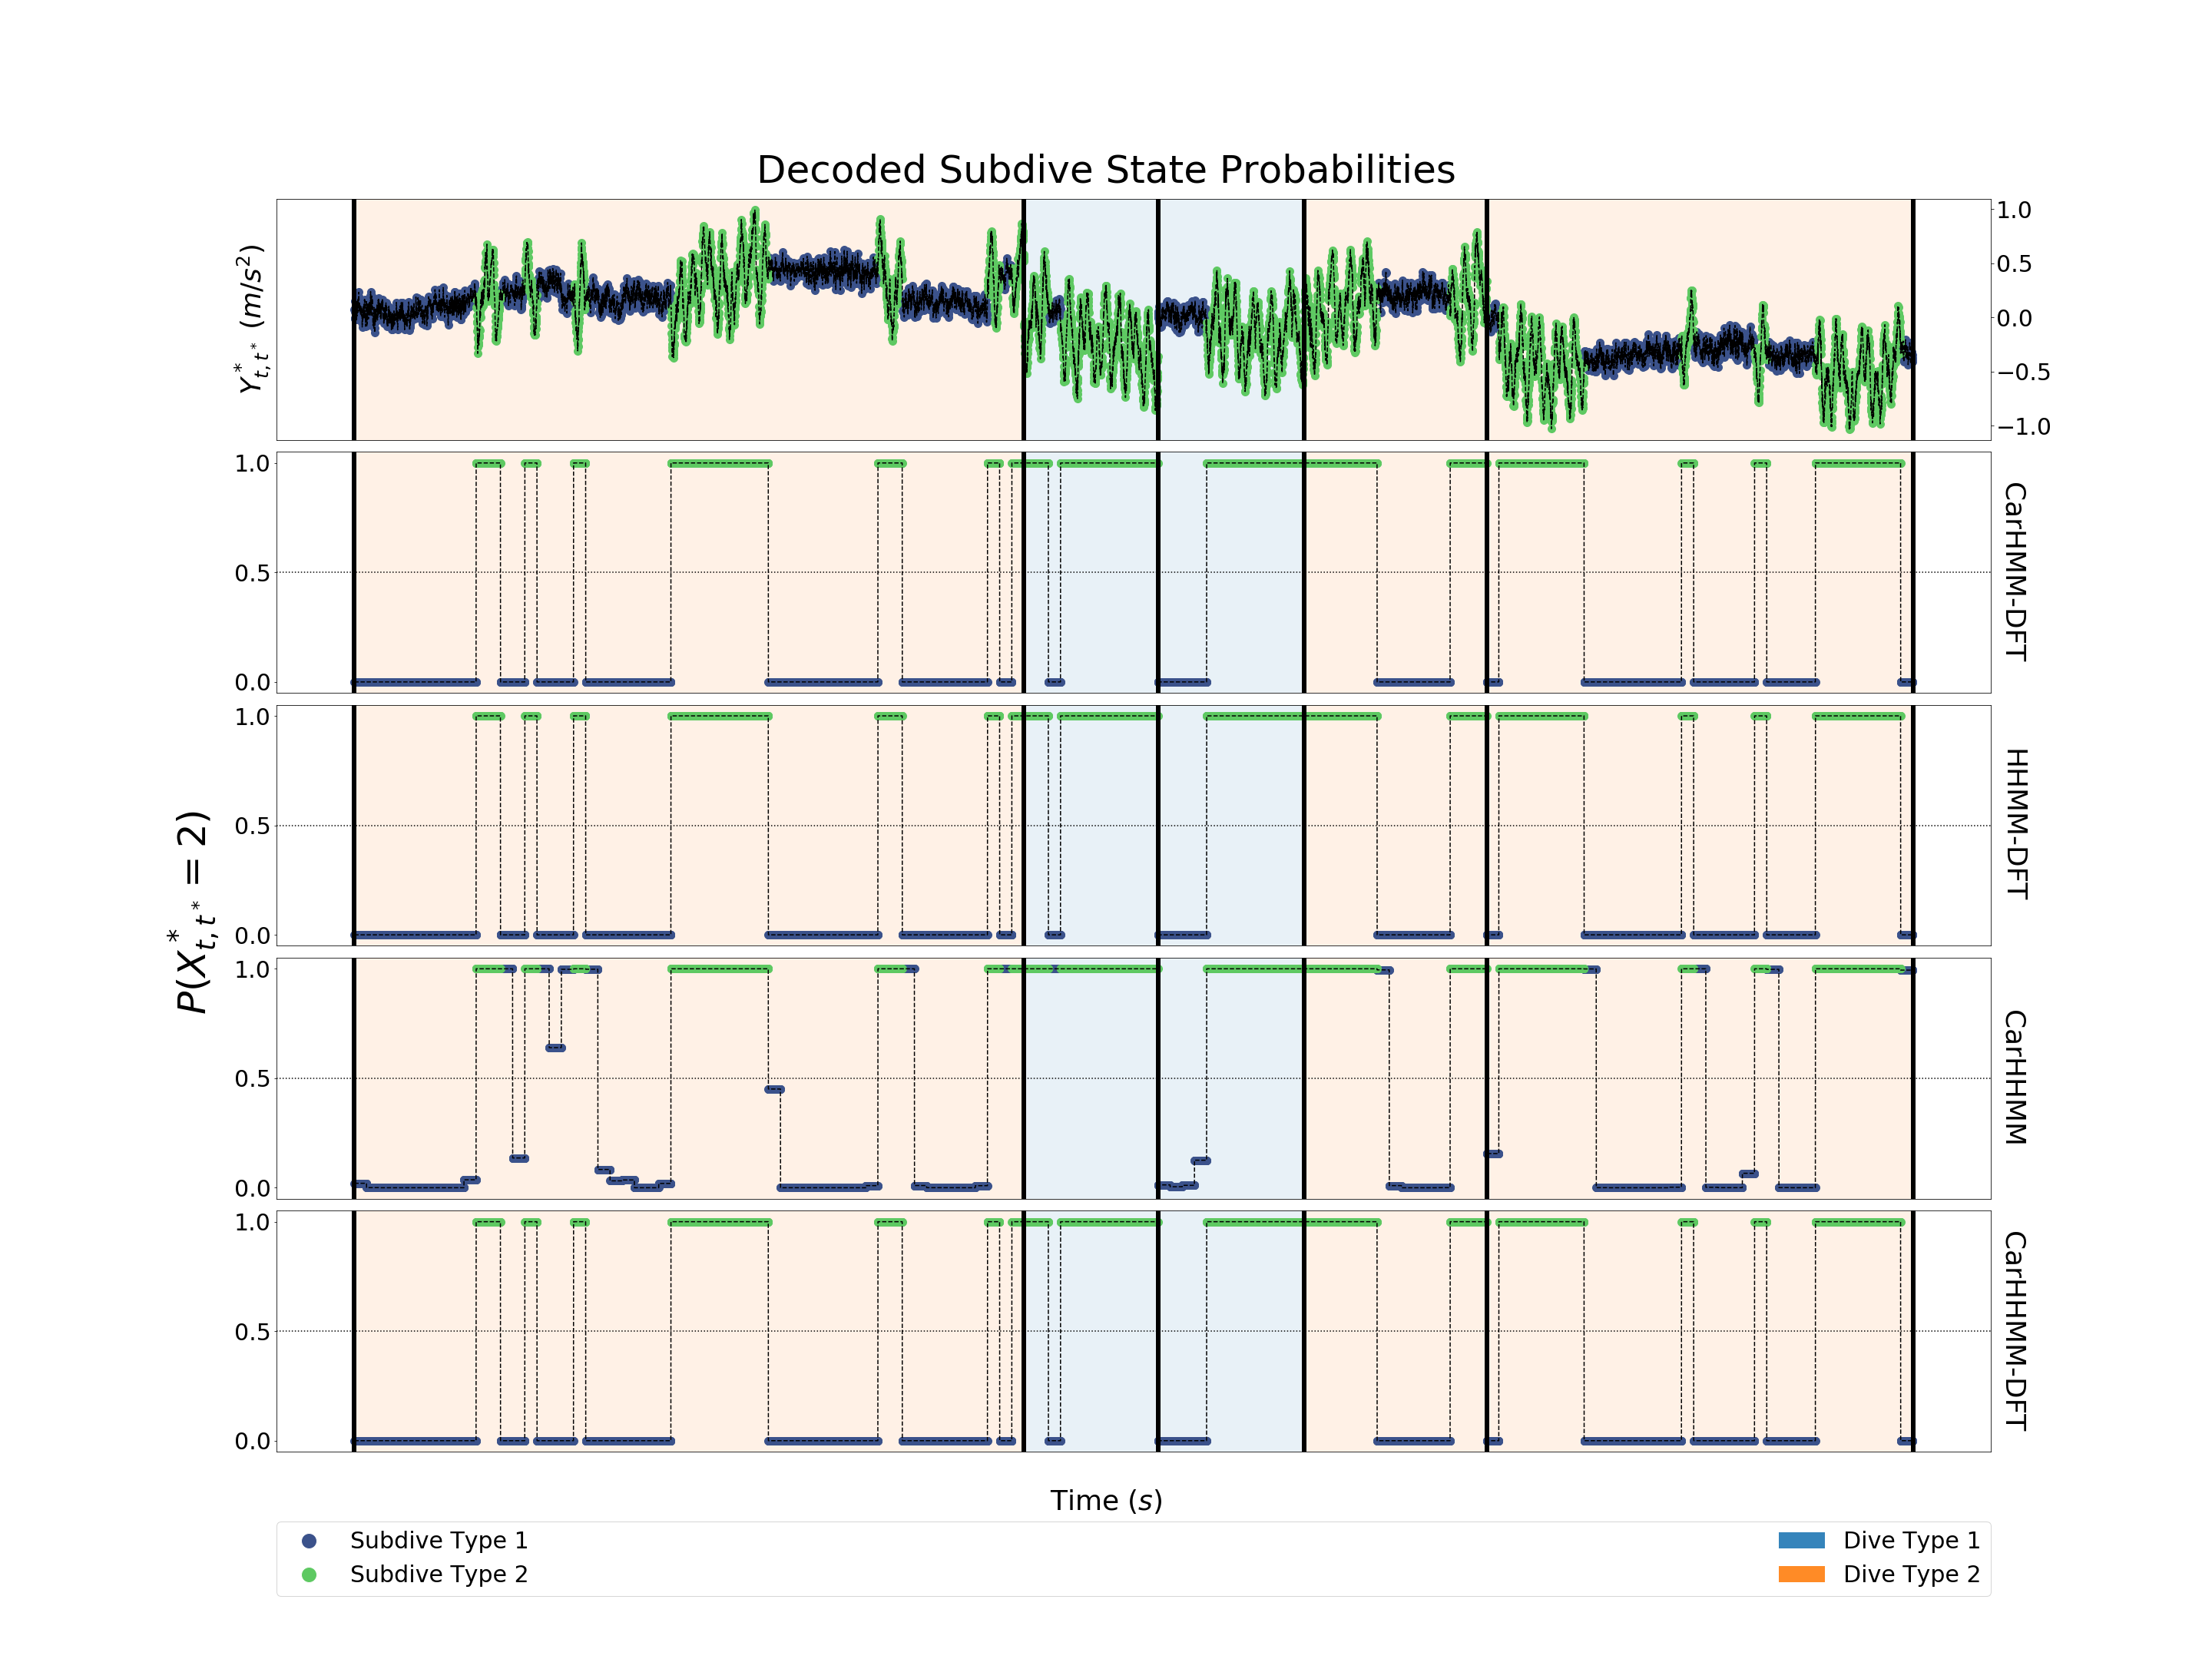
\includegraphics[width=5in]{Plots/Posterior_Fine_States.png}
        \caption{Fine-scale hidden process}
    \end{subfigure}
	\caption{Decoded state probabilities of each model. The color of the line corresponds to the true fine-scale state of the sub-dive process, while the color of the background corresponds to the true dive type of the simulated whale.}
	\label{fig:acc}
\end{figure}

%%% dive duration %%%
For the emission distributions of dive duration, estimates of standard error using the observed fisher information tended to be underestimates due to correlation between $\hat \mu$ and $\hat \sigma$. In addition, $\hat \sigma$ tends to underestimate $\sigma$ for all models, which is a finding consistent with properties of MLEs, especially because the sample size for a particular dive type is approximately 50 for each simulation. The CarHMM model in particular severely underestimates $\sigma$. This is likely due to the fact that dive duration follows a mixture of gammas rather than a gamma distribution, and the CarHMM does not have the machinary to capture this fact. A full table of parameter estimates for all models is shown in (table \ref{table:dive_duration}).


%%% Acceleration %%%
For acceleration ($Z^{*(1)}$), both the CarHMM and the CarHHMM2 regularly converged to the correct parameters with very little standard error. Note, however, that both have relatively large observed fisher standard error in $\hat \mu$. This likely is due to the very large autocorrelation terms ($\phi^{(1)} = 0.99$ and $\phi^{(2)} = 0.95$) since as $\phi \to 1$, the value of $\mu$ does not matter in the likelihood evaluation as $\phi \to 1$ implies that $\mathbb{E}(Z^{*(1)}_{t,s^*}) = \phi*(Z^{*(1)}_{t,s^*-1}) + (1-\phi)\mu \to Z^{*(1)}_{t,s^*-1}$. The HHMM overestimates the variance of $Z^{*(1)}$ since it does not incorporate auto-correlation into the emission distribution of $Z^{*(1)}$, and the CarHHMM1 has large biases in many of its parameter estimates, especially in subdive state 2, because it sees the ``wigliness" of the acceleration data as raw acceleration rather than as Fourier modes, which deflates the value of $\hat \phi$ and inflates the value of $\hat \sigma$. See (table \ref{table:acceleration}) for a detailed breakdown of parameter values for acceleration emission distributions.

%%% FoVeDBA %%%

Finally, the distribution of parameters for the Fourier sums ($Z^{*(2)}$) for all models (except for the CarHHMM1) converge to the correct values, and the observed fisher information standard errors are in line with the empirical standard error. The distribution of $Z^{*(2)}$ is very different between subdive states 1 and 2, so the signal is therefore very easy for each model to pick up on. (Table \ref{table:FoVeDBA}) shows a detailed breakdown of the emission distribution of $Z^{*(2)}$ for all models.

\textcolor{red}{I also have similar tables for $\Gamma$ and $\Gamma^*$, and I also have plots corresponding to each table. For example, I have included figure \ref{fig:MLE_dist} as an example below for the emission distribution of the MLEs for dive duration of the CarHMM. Should I use those instead? But there are just SO many plots (4 models * 3 observations * 2 states = 24 plots)}

\begin{figure}[!ht]
	\centering
	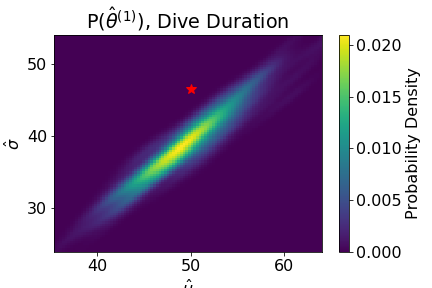
\includegraphics[width=5in]{../Plots/hmm_FV_MLE_density_dive_duration_-1.png}
	\caption{\textcolor{red}{KDE plot of $\hat \mu$ and $\hat \sigma$ for the dive duration emission distribution for the CarHMM. This plot is for Marie and Nancy to look over.}}
	\label{fig:MLE_dist}
\end{figure}



%%% Accuracy %%%

\begin{table}[]
\centering
\caption{Accuracies and run times for all models. All reported values are averages, and $\pm$ refers to the standard deviation.}
\scalebox{0.8}{
\begin{tabular}{ccccccc}
Model                      & \multicolumn{1}{c}{Training Time (Minutes)} & \multicolumn{1}{c}{Dive Type} & \multicolumn{1}{c}{Subdive Type} & \multicolumn{1}{c}{Dive Accuracy} & \multicolumn{1}{c}{Subdive Accuracy}  \\ \hline
\multirow{5}{*}{CarHMM}    & \multirow{5}{*}{$15.74 \pm 2.46$}   & Both                          & Both                             & -------------                     & $1.00 \pm 0.00$                       \\
                           &                                    & 1                             & 1                                & \multirow{2}{*}{-------------}    & $1.00 \pm 0.00$                       \\ 
                           &                                    & 1                             & 2                                &                                   & $1.00 \pm 0.00$                       \\ 
                           &                                    & 2                             & 1                                & \multirow{2}{*}{-------------}    & $1.00 \pm 0.00$                       \\ 
                           &                                    & 2                             & 2                                &                                   & $1.00 \pm 0.00$                       \\ \hline 
\multirow{5}{*}{HHMM}      & \multirow{5}{*}{$82.43 \pm 11.48$}   & Both                          & Both                             & $0.94 \pm 0.02$                   & $1.00 \pm 0.00$                       \\
                           &                                    & 1                             & 1                                & \multirow{2}{*}{$0.94\pm0.03$}    & $1.00 \pm 0.00$                       \\ 
                           &                                    & 1                             & 2                                &                                   & $1.00 \pm 0.00$                       \\ 
                           &                                    & 2                             & 1                                & \multirow{2}{*}{$0.94\pm0.03$}    & $1.00 \pm 0.00$                       \\ 
                           &                                    & 2                             & 2                                &                                   & $1.00 \pm 0.00$                       \\ \hline
\multirow{5}{*}{CarHHMM1}  & \multirow{5}{*}{$70.85 \pm 15.89$}   & Both                          & Both                             & $0.91 \pm 0.03$                   & $0.89 \pm 0.02$                       \\
                           &                                    & 1                             & 1                                & \multirow{2}{*}{$0.87\pm0.04$}    & $0.44 \pm 0.12$                       \\ 
                           &                                    & 1                             & 2                                &                                   & $1.00 \pm 0.00$                       \\ 
                           &                                    & 2                             & 1                                & \multirow{2}{*}{$0.95\pm0.03$}    & $0.81 \pm 0.04$                       \\ 
                           &                                    & 2                             & 2                                &                                   & $1.00 \pm 0.00$                       \\ \hline
\multirow{5}{*}{CarHHMM2}  & \multirow{5}{*}{$81.22 \pm 16.10$}   & Both                          & Both                             & $0.94 \pm 0.02$                   & $1.00 \pm 0.00$                       \\
                           &                                    & 1                             & 1                                & \multirow{2}{*}{$0.94\pm0.03$}    & $1.00 \pm 0.00$                       \\ 
                           &                                    & 1                             & 2                                &                                   & $1.00 \pm 0.00$                       \\ 
                           &                                    & 2                             & 1                                & \multirow{2}{*}{$0.94\pm0.03$}    & $1.00 \pm 0.00$                       \\ 
                           &                                    & 2                             & 2                                &                                   & $1.00 \pm 0.00$                       \\ \hline
\end{tabular}
}
\label{table:accuracy}
\end{table}

%%% dive duration %%%

\begin{table}[]
\centering
\caption{Estimates and standard errors of parameters for dive duration distribution for all four models. All reported values are averages, except for the Fisher observed standard error, which are medians. $\pm$ refers to the IQR.}
\scalebox{0.9}{
\begin{tabular}{ccccccc}
Model                      & \multicolumn{1}{c}{Parameter} & \multicolumn{1}{c}{Dive Type} & \multicolumn{1}{c}{Estimate} & \multicolumn{1}{c}{Bias} & \multicolumn{1}{c}{Empirical SE} & \multicolumn{1}{c}{Observed Fischer SE}           \\ \hline
\multirow{4}{*}{CarHMM}    & \multirow{2}{*}{$\mu$}        & 1                             & $49.72$                         & $-0.28$                     & $4.78$                             & $2.47 \pm 0.34$                             \\
                           &                               & ---                           & ---                            & ---                        & ---                                & ---                                         \\
                           & \multirow{2}{*}{$\sigma$}     & 1                             & $39.00$                         & $-7.51$                     & $5.05$                             & $2.50 \pm 0.40$                             \\
                           &                               & ---                           & ---                            & ---                        & ---                                & ---                                         \\ \hline
\multirow{4}{*}{HHMM}      & \multirow{2}{*}{$\mu$}        & 1                             & $19.99$                         & $-0.01$                     & $0.75$                             & $0.69 \pm 0.11$                             \\
                           &                               & 2                             & $79.85$                         & $-0.15$                     & $8.05$                             & $5.85 \pm 1.10$                             \\
                           & \multirow{2}{*}{$\sigma$}     & 1                             & $4.90$                         & $-0.10$                     & $0.61$                             & $0.53 \pm 0.10$                             \\
                           &                               & 2                             & $48.74$                         & $-1.26$                     & $6.50$                             & $5.15 \pm 1.02$                             \\ \hline
\multirow{4}{*}{CarHHMM 1} & \multirow{2}{*}{$\mu$}        & 1                             & $19.91$                         & $-0.09$                     & $0.77$                             & $0.71 \pm 0.12$                             \\
                           &                               & 2                             & $75.80$                         & $-4.20$                     & $7.72$                             & $5.32 \pm 0.98$                             \\
                           & \multirow{2}{*}{$\sigma$}     & 1                             & $4.73$                         & $-0.27$                     & $0.59$                             & $0.55 \pm 0.10$                             \\
                           &                               & 2                             & $49.48$                         & $-0.52$                     & $6.26$                             & $4.79 \pm 0.93$                             \\ \hline
\multirow{4}{*}{CarHHMM 2} & \multirow{2}{*}{$\mu$}        & 1                             & $19.99$                         & $-0.01$                     & $0.75$                             & $0.69 \pm 0.12$                             \\
                           &                               & 2                             & $79.85$                         & $-0.15$                     & $8.05$                             & $5.85 \pm 1.10$                             \\
                           & \multirow{2}{*}{$\sigma$}     & 1                             & $4.90$                         & $-0.10$                     & $0.61$                             & $0.53 \pm 0.10$                             \\
                           &                               & 2                             & $48.74$                         & $-1.26$                     & $6.50$                             & $5.15 \pm 1.02$                             
\end{tabular}
}
\label{table:dive_duration}
\end{table}


%%% Acceleration %%%

\begin{table}[]
\centering
\caption{Estimates and standard errors of parameters for $Z^{*(1)}_{t,s^*}$ for all four models. All reported values are averages, except for the Fisher observed standard error, which are medians. $\pm$ refers to the IQR.}
\scalebox{0.8}{
\begin{tabular}{ccccccc}
Model                      & \multicolumn{1}{c}{Parameter} & \multicolumn{1}{c}{Subdive Type} & \multicolumn{1}{c}{Estimate} & \multicolumn{1}{c}{Bias} & \multicolumn{1}{c}{Empirical SE} & \multicolumn{1}{c}{Observed Fischer SE}        \\ \hline
\multirow{6}{*}{CarHMM}    & \multirow{2}{*}{$\mu$}        & 1                             & $0.00$                         & $0.00$                     & $0.00$                             & $0.14 \pm 0.13$                             \\
                           &                               & 2                             & $0.00$                         & $0.00$                     & $0.01$                             & $0.06 \pm 0.02$                             \\
                           & \multirow{2}{*}{$\sigma$}     & 1                             & $0.05$                         & $-0.00$                     & $0.00$                             & $0.00 \pm 0.00$                             \\
                           &                               & 2                             & $0.10$                         & $-0.00$                     & $0.00$                             & $0.00 \pm 0.00$                             \\ 
                           & \multirow{2}{*}{$\phi$}       & 1                             & $0.99$                         & $-0.00$                     & $0.01$                             & $0.01 \pm 0.00$                             \\
                           &                               & 2                             & $0.95$                         & $-0.00$                     & $0.01$                             & $0.01 \pm 0.00$                             \\ \hline
\multirow{6}{*}{HHMM}      & \multirow{2}{*}{$\mu$}        & 1                             & $-0.01$                         & $-0.01$                     & $0.02$                             & $0.01 \pm 0.00$                             \\
                           &                               & 2                             & $-0.00$                         & $-0.00$                     & $0.02$                             & $0.01 \pm 0.00$                             \\
                           & \multirow{2}{*}{$\sigma$}     & 1                             & $0.25$                         & $0.20$                     & $0.04$                             & $0.00 \pm 0.00$                             \\
                           &                               & 2                             & $0.24$                         & $0.14$                     & $0.03$                             & $0.00 \pm 0.00$                             \\ 
                           & \multirow{2}{*}{$\phi$}       & 1                             & ------                         & ------                     & ------                             & ------                                      \\
                           &                               & 2                             & ------                         & ------                     & ------                             & ------                                      \\ \hline
\multirow{6}{*}{CarHHMM 1} & \multirow{2}{*}{$\mu$}        & 1                             & $0.00$                         & $0.00$                     & $0.00$                             & $0.08 \pm 0.04$                             \\
                           &                               & 2                             & $-0.01$                         & $-0.01$                     & $0.01$                             & $0.01 \pm 0.00$                             \\
                           & \multirow{2}{*}{$\sigma$}     & 1                             & $0.05$                         & $0.00$                     & $0.04$                             & $0.00 \pm 0.00$                             \\
                           &                               & 2                             & $0.27$                         & $0.17$                     & $0.01$                             & $0.00 \pm 0.00$                             \\ 
                           & \multirow{2}{*}{$\phi$}       & 1                             & $0.97$                         & $-0.02$                     & $0.10$                             & $0.00 \pm 0.00$                             \\
                           &                               & 2                             & $0.49$                         & $-0.46$                     & $0.05$                             & $0.02 \pm 0.00$                             \\ \hline
\multirow{6}{*}{CarHHMM 2} & \multirow{2}{*}{$\mu$}        & 1                             & $0.00$                         & $0.00$                     & $0.00$                             & $0.13 \pm 0.12$                             \\
                           &                               & 2                             & $0.00$                         & $0.00$                     & $0.00$                             & $0.06 \pm 0.02$                             \\
                           & \multirow{2}{*}{$\sigma$}     & 1                             & $0.05$                         & $-0.00$                     & $0.00$                             & $0.00 \pm 0.00$                             \\
                           &                               & 2                             & $0.10$                         & $-0.00$                     & $0.00$                             & $0.00 \pm 0.00$                             \\ 
                           & \multirow{2}{*}{$\phi$}       & 1                             & $0.99$                         & $-0.00$                     & $0.01$                             & $0.01 \pm 0.00$                             \\
                           &                               & 2                             & $0.95$                         & $-0.00$                     & $0.01$                             & $0.01 \pm 0.00$                             \\ \hline
\end{tabular}
}
\label{table:acceleration}
\end{table}


%%% FoVeDBA %%%

\begin{table}[]
\centering
\caption{Estimates and standard errors of parameters for $Z^{*(2)}_{t,s^*}$ for all four models. All reported values are averages, except for the Fisher observed standard error, which are medians. $\pm$ refers to the IQR.}
\scalebox{0.8}{
\begin{tabular}{ccccccc}
Model                      & \multicolumn{1}{c}{Parameter} & \multicolumn{1}{c}{Subdive Type} & \multicolumn{1}{c}{Estimate} & \multicolumn{1}{c}{Bias} & \multicolumn{1}{c}{Empirical SE} & \multicolumn{1}{c}{Observed Fischer SE}        \\ \hline
\multirow{4}{*}{CarHMM}    & \multirow{2}{*}{$\mu$}        & 1                             & $10.10$                         & $-0.00$                     & $0.09$                             & $0.08 \pm 0.01$                             \\
                           &                               & 2                             & $305.97$                         & $0.03$                     & $0.54$                             & $0.51 \pm 0.03$                             \\
                           & \multirow{2}{*}{$\sigma$}     & 1                             & $3.18$                         & $-0.00$                     & $0.07$                             & $0.06 \pm 0.01$                             \\
                           &                               & 2                             & $17.46$                         & $-0.03$                     & $0.37$                             & $0.36 \pm 0.02$                             \\ \hline
\multirow{4}{*}{HHMM}      & \multirow{2}{*}{$\mu$}        & 1                             & $10.10$                         & $-0.00$                     & $0.09$                             & $0.08 \pm 0.01$                             \\
                           &                               & 2                             & $305.97$                         & $0.03$                     & $0.54$                             & $0.51 \pm 0.03$                             \\
                           & \multirow{2}{*}{$\sigma$}     & 1                             & $3.18$                         & $-0.00$                     & $0.07$                             & $0.06 \pm 0.01$                             \\
                           &                               & 2                             & $17.46$                         & $-0.03$                     & $0.37$                             & $0.36 \pm 0.02$                             \\ \hline
\multirow{4}{*}{CarHHMM 1} & \multirow{2}{*}{$\mu$}        & 1                             & ------                         & ------                     & ------                             & ------                                      \\
                           &                               & 2                             & ------                         & ------                     & ------                             & ------                                      \\
                           & \multirow{2}{*}{$\sigma$}     & 1                             & ------                         & ------                     & ------                             & ------                                      \\
                           &                               & 2                             & ------                         & ------                     & ------                             & ------                                      \\ \hline
\multirow{4}{*}{CarHHMM 2} & \multirow{2}{*}{$\mu$}        & 1                             & $10.10$                         & $-0.00$                     & $0.09$                             & $0.08 \pm 0.01$                             \\
                           &                               & 2                             & $305.97$                         & $0.03$                     & $0.54$                             & $0.51 \pm 0.03$                             \\
                           & \multirow{2}{*}{$\sigma$}     & 1                             & $3.18$                         & $-0.00$                     & $0.07$                             & $0.06 \pm 0.01$                             \\
                           &                               & 2                             & $17.46$                         & $-0.03$                     & $0.37$                             & $0.36 \pm 0.02$                             
\end{tabular}
}
\label{table:FoVeDBA}
\end{table}

